
\begin{document}
	\title{COMS3008A Assignment -- Report}
	\author{Claudio Da Mata - 2128358}
	\date{23-10-2022} 
	\maketitle 
	%\thispagestyle{empty}
	\pagestyle{fancy}
	\fancyhf{}
	\fancyhead[R]{\thepage}
	\fancyhead[L]{COMS3008A Assinment}
	%\vskip 3mm 
	%\pagenumbering{roman}
	%\newpage
	\pagenumbering{arabic} 
	\graphicspath{ {./pics/} }
	\bibliographystyle{elsarticle-num}
	
	\section{Problem 1: Parallel Scan}
	\begin{itemize}
		\item  Given a set of elements, $[a_0,a_1,\dotsm,a_{n-1}]$, the scan operation associated with addition operator for this input is the output set $[a_0,(a_0+a_1),\dotsm,(a_0+a_1+\dotsm+a_{n-1})]$. 
		\item For example, the input set is $[2,1,4,0,3,7,6,3]$, then the scan with addition operator of this input is $[2,3,7,7,10,17,23,26]$. 
	\end{itemize}

	\subsection{Serial Implementation:}
	Firstly I started off with the baseline implementation of serial scan operation given in Listing~\ref{listing:ls_serial_scan}
	\begin{lstlisting}[caption={Sequential algorithm for computing scan operation with ‘+’ operator\cite{PrefixSumArray}.}, label={listing:ls_serial_scan}]
		void scan(int out[], int in[], int N){
			out[0] = in[0];
			
			for(int i=1; i<N; i++) {
				out[i] = in[i] + out[i-1];
			}
		}
	\end{lstlisting}
	
	This got me a baseline average time to measure and compare parallel implementations. I ran the operation (10 times, taking average) on arrays ranging in sizes from $1000$ to $50,000$ with intervals of $1000$ given in Figure~\ref{fig:fig_serial_scan}
	\begin{figure}[!htb]
		\centering
		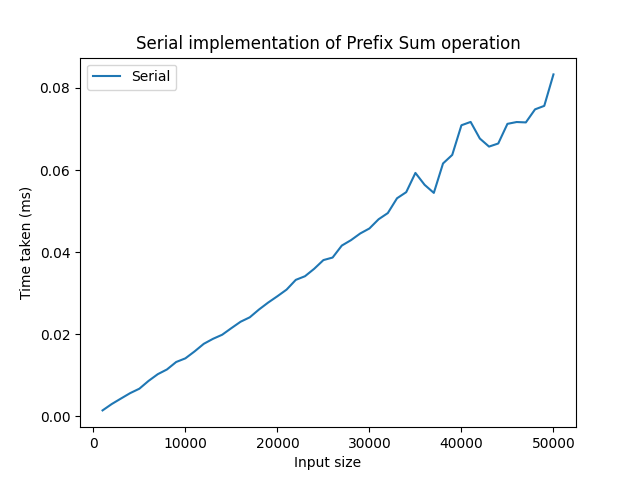
\includegraphics[width=0.6\linewidth]{serial_scan.png}
		\caption{Serial scan operation average times}
		\label{fig:fig_serial_scan}
	\end{figure}
	
	\newpage
	\subsection{OpenMP Parallel Implementation:}
	Next I implented the scan operation within OpenMP's interface. The algorithm I used is based off the Blelloch\cite{Prefixsumwiki} work-effecient algorithm given in Listing~\ref{listing:ls_scan_omp}
	\begin{lstlisting}[caption={OpenMP Parallel algorithm for computing scan operation\cite{PrefixsumCSE}.}, label={listing:ls_scan_omp}]
		void scan(int out[], int in[], int N){
			int nthr, *z, *x = out;
			#pragma omp parallel num_threads(4)
			{
				int i;
				#pragma omp single
				{
					nthr = omp_get_num_threads();
					z = malloc(sizeof(int)*nthr+1);
					z[0] = 0;
				}
				
				int tid = omp_get_thread_num();
				int sum = 0;
				#pragma omp for schedule(static)
				for(i=0; i<N; i++) {
					sum += in[i];
					x[i] = sum;
				}
				
				z[tid+1] = sum;
				#pragma omp barrier
				
				int offset = 0;
				for(i=0; i<(tid+1); i++) {
					offset += z[i];
				}
				
				#pragma omp for schedule(static)
				for(i=0; i<N; i++){
					x[i] += offset;
				}
			}
			free(z);
		}
	\end{lstlisting}

	The algorithm works as follows:
	\begin{itemize}
		\item Start omp parallel
		\item Initiate a 'single' construct which allows only one thread to run the code
		\item Inside single should declare the size of the temp array and set $element[0] = 0$
		\item After the single construct, get current threadID and initialize $sum =0$
		\item Begin an omp for contruct with schedule(static)
		\item Inside the for loop (from $0$ to $N-1$), $sum +=$ the input array at $i$, and set the output array at $i$ equal to the new $sum$
		\item After the for loop, set temp array at $[threadID+1]$ equal to $sum$
		\item Declare a Barrier construct which forces all threads to wait until other threads finish computation
		\item Set offset $= 0$ 
		\item Begin a regular for loop that sums all elements of the temp array to $offset$, only adding elements that each specific thread has computed itself
		\item Begin an omp for construct with schedule(static) again, from $i = 0$ to $N-1$
		\item sum output array element $i$ with offset
		\item Finish off pragma omp and then free the temp array from memory
	\end{itemize}
	
	I experimented with different number of threads running and managed to narrow it down to thread counts of $2,4,6$ given in Figure~\ref{fig:fig_scan_omp_comparison}
	
	With 2 threads running there is no noticeable speedup compared to serial implementation. With 4 and 6 threads running there is significant speedup compared to serial implementation. While input size n increases, 4 threads performs slightly better than 6 threads. Thus I choose 4 threads as my optimal implementation of OpenMP parallelization.
	\begin{figure}[!htb]
		\centering
		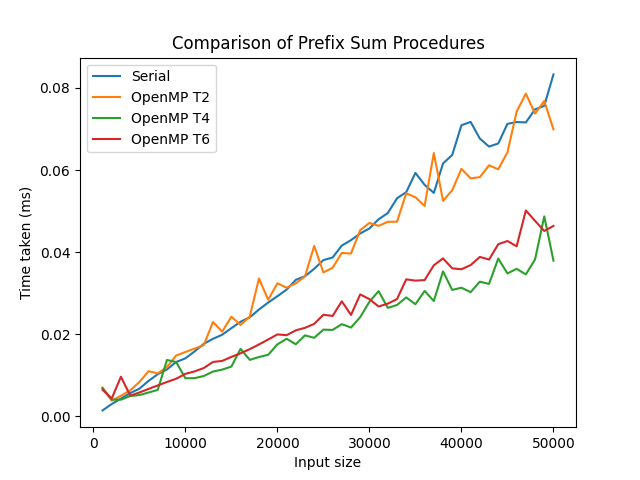
\includegraphics[width=0.6\linewidth]{scan_omp_comparison.png}
		\caption{OpenMP Parallel scan operation average times for different thread counts}
		\label{fig:fig_scan_omp_comparison}
	\end{figure}
	
	\subsection{MPI Parallel Implementation:}
	Next I implented the scan operation within MPI's interface. The algorithm I used is based off the Blelloch\cite{Prefixsumwiki} prescan algorithm given in Listing~\ref{listing:ls_scan_mpi}
	\begin{lstlisting}[caption={MPI Parallel algorithm for computing scan operation\cite{PrefixsumMPI}.}, label={listing:ls_scan_mpi}]
		MPI_Init(&argc, &argv); //Initialize MPI
		
		MPI_Comm_rank(MPI_COMM_WORLD, &my_rank);
		MPI_Comm_size(MPI_COMM_WORLD, &comm_size);
		
		MPI_Barrier(MPI_COMM_WORLD);
		
		size_t num_per_proc = n / comm_size;
		int sum;
		
		start_find_sum(my_rank, comm_size, data, num_per_proc,
		&sum);
		start_find_psum(my_rank, comm_size, data, num_per_proc,
		sum);
		
		MPI_Barrier(MPI_COMM_WORLD);
		
		MPI_Finalize(); //Close MPI
	\end{lstlisting}
	
	The essence of the algorith comes from the start\textunderscore find\textunderscore sum() and start\textunderscore find\textunderscore psum() functions.
	
	The algorithm works as follows:
	\begin{itemize}
		\item Start MPI
		\item Get comm rank and size
		\item Barrier that forces all threads to wait
		\item Set num per proc equal to array size $n / comm size$. This dictates how many numbers each thread will compute the sums of
		\item Call start\textunderscore find\textunderscore sum() function
		\begin{itemize}
			\item The algoritem works like a binary tree with levels
			\item Gets MPI\textunderscore Status
			\item Sums input array elements from $0$ to $numPerProc$
			\item Begin for loop from $level =0$ to $log_{2}(comm size)$
			\item Inside the loop set $position = rank / level^{2}$
			\item If $position$ is even, receives the $sendersSum$ (with $senderRank = rank + level^2$) and adds to total $sum$
			\item If $position$ is odd, sends total $sum$ to receiver with $senderRank = rank - level^2$, then kills current thread
			\item Before for loop ends, calls Barrier so all threads wait
		\end{itemize}
		\item Call start\textunderscore find\textunderscore psum() function
		\begin{itemize}
			\item The algorithm works like a binary tree with levels
			\item Gets MPI\textunderscore Status
			\item If $rank == 0$, sets $psum = sum$
			\item Begin for loop from $level = log_2(comm size) -1$ down to $0$
			\item If process is on current level:
			\item Set $position = rank / level^2$
			\item If $position$ is even this means this process was the parent of $sendingRank$, and so first sets $senderRank = rank + level^2$, then sends $psum$, then receives the $senderSum$ and finally subtracts $psum$ by $senderSum$
			\item If $position$ is odd, sets $receivingRank = rank - level^2$, then receives $psum$ from parent, and then sends $sum$ with $receivingRank$
			\item Before for loop ends, calls Barrier so all threads wait
			\item After the loop ends, put the $prefixSums$ associated with this process in the input array
		\end{itemize}
		\item Calls Barrier so all threads wait
		\item Ends MPI
	\end{itemize}
	
	With start\textunderscore find\textunderscore sum() and start\textunderscore find\textunderscore psum() functions given respectively by Listing~\ref{listing:ls_findsum} and Listing~\ref{listing:ls_findpsum}
	\begin{lstlisting}[caption={start\textunderscore find\textunderscore sum()}, label={listing:ls_findsum}]
		void start_find_sum(int rank, int mysize, int* in, 
							size_t num_per_proc, int* overall_sum){
			MPI_Status status;
			
			int sum = find_sum(in, num_per_proc);
			
			int still_alive = 1;
			int level;
			
			for (level = 0; level < (int)log2(mysize); level++) {
				if (still_alive) {
					int position = rank / (int)pow(2, level);
					
					if (position % 2 == 0) {
						// I am a receiver
						int sender_sum;
						int sending_rank = rank + (int)pow(2, level);
						
						MPI_Recv(&sender_sum, 1, MPI_INT, sending_rank,
						0, MPI_COMM_WORLD, &status);
						
						sum += sender_sum;
					}else {
						// I am a sender
						int receiving_rank = rank - (int)pow(2, level);
						
						MPI_Send(&sum, 1, MPI_INT, receiving_rank, 0,
						MPI_COMM_WORLD);
						still_alive = 0;
					}
				}
				MPI_Barrier(MPI_COMM_WORLD);
			}
			*overall_sum = sum;
		}
	\end{lstlisting}
	\begin{lstlisting}[caption={start\textunderscore find\textunderscore psum()}, label={listing:ls_findpsum}]
		void start_find_psum(int rank, int mysize, int* in,
							size_t num_per_proc, int sum){
			int psum;
			int level;
			MPI_Status status;  
			
			if (rank == 0) {
				psum = sum;
			}
			for (level = (int)log2(mysize) - 1; level >= 0; level--) {
				// only trigger the processes on the current level
				if (level == 0 || rank % (int)pow(2, level) == 0) {
					int position = rank / (int)pow(2, level);
					
					if (position % 2 == 0) {
						int sender_sum;
						int sending_rank = rank + (int)pow(2, level);
						
						MPI_Send(&psum, 1, MPI_INT,
						sending_rank, // RIGHT CHILD
						0, MPI_COMM_WORLD);
						
						MPI_Recv(&sender_sum, 1, MPI_INT,
						sending_rank, 0, MPI_COMM_WORLD, &status);

						// psum <- (prefix sum of parent) - (sum of sibling)
						psum -= sender_sum;
					}else{
						int receiving_rank = rank - (int)pow(2, level);
						
						MPI_Recv(&psum, 1, MPI_INT,
						receiving_rank, // PARENT
						0, MPI_COMM_WORLD, &status);
						
						// send sum to receiving_rank so it can fix its sum
						MPI_Send(&sum, 1, MPI_INT,
						receiving_rank, 0, MPI_COMM_WORLD);
					}
				}
				MPI_Barrier(MPI_COMM_WORLD);
			}
			// put the prefix sums associated with this node in input array
			int next_sum = in[num_per_proc-1];
			in[num_per_proc-1] = psum;
			
			for (int j = num_per_proc - 2; j >= 0; j--) {
				int next_sum_tmp = in[j];
				
				in[j] = in[j+1] - next_sum;
				
				next_sum = next_sum_tmp;
			}
		}
	\end{lstlisting}
	
	I experimented with different number of threads running and managed to narrow it down to thread counts of $2,4,8$ given in Figure~\ref{fig:fig_scan_mpi_comparison}
	
	With 2 threads running there is noticeably worse running time compared to serial implementation. With 4 and 8 threads running there is significant speedup compared to serial implementation. With smaller input sizes n, 4 threads performs better than 8 threads, but as n increases, perfermance between 4 threads and 8 threads stays relatively the same. Thus I choose 4 threads as my optimal implementation of MPI parallelization.
	\begin{figure}[!htb]
		\centering
		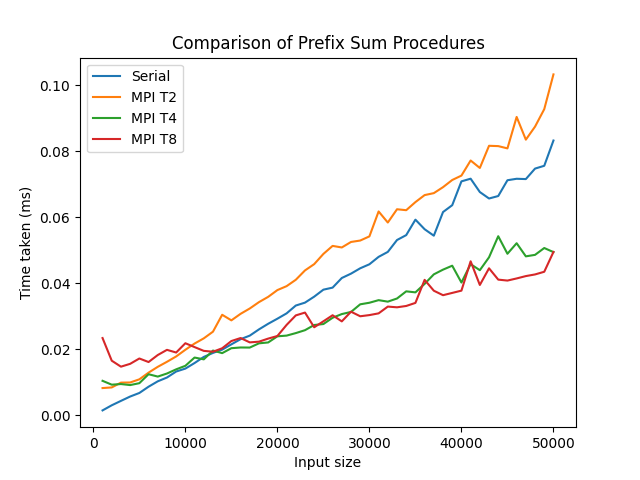
\includegraphics[width=0.6\linewidth]{scan_mpi_comparison.png}
		\caption{MPI Parallel scan operation average times for different thread counts}
		\label{fig:fig_scan_mpi_comparison}
	\end{figure}

	\subsection{Validation:}
	Checking if elements are correclty summed, through running $run.sh$ given in Figure~\ref{fig:fig_scan_validation}
	\begin{figure}[!htb]
		\centering
		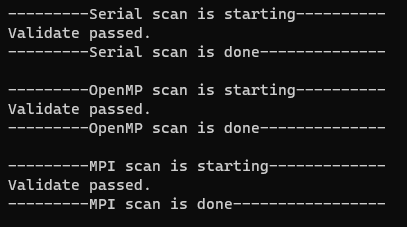
\includegraphics[width=0.5\linewidth]{scan_validation.png}
		\caption{Validation of scan operations}
		\label{fig:fig_scan_validation}
	\end{figure}

	\subsection{Conclusions:}
	After comparing the results from serial, optimal OpenMP (with 4 threads) and optimal MPI (with 4 threads), I can make the conclusion that serial performs the best at very small array size n. While at large n, both OpenMP and MPI have significant speedup from serial, OpenMP performs consistently better than MPI.
	Comparisons given in Figure~\ref{fig:fig_scan_comparison}
	\begin{figure}[!htb]
		\centering
		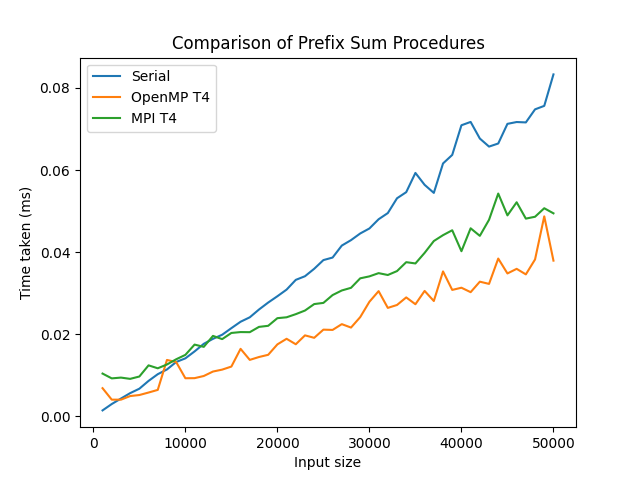
\includegraphics[width=0.6\linewidth]{scan_comparison.png}
		\caption{Comparison of all scan operations}
		\label{fig:fig_scan_comparison}
	\end{figure}

	\section{Problem 2: Parallel Bitonic Sort}
	Not applicable, working alone.
	
	\section{Problem 3: Parallel Graph Algorithm}
	Implementing Dijkstra’s Single Source Shortest Path (SSSP) Algorithm. An example problem is given in Figure~\ref{fig:sp_fig1}.
	\begin{figure}[!htb]
		\centering
		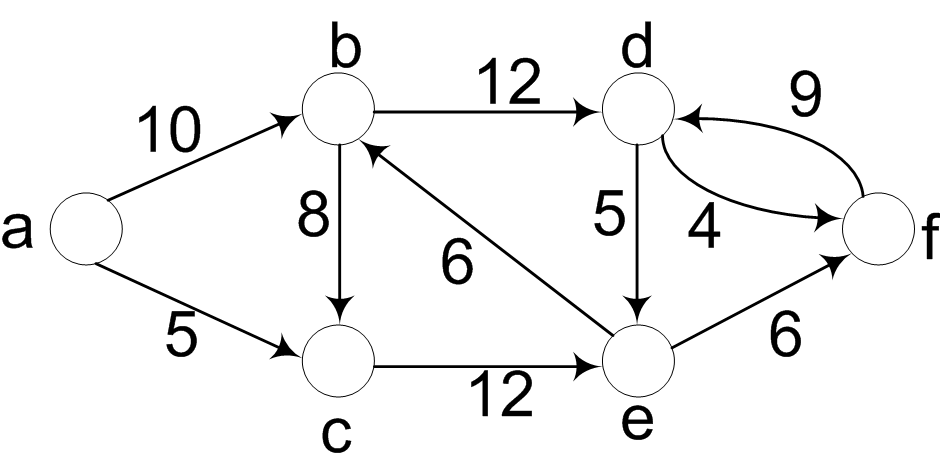
\includegraphics[width=0.3\linewidth]{sp_fig1.png}
		\caption{A directed graph}\label{fig:sp_fig1}
	\end{figure}
	
	\subsection{Serial Implementation:}
	Firstly I started off with the baseline implementation of serial SSSP algorithm given in Listing~\ref{listing:ls_serial_sssp}
	\begin{lstlisting}[caption={Sequential algorithm for Dijkstra’s SSSP\cite{SSSP}.}, label={listing:ls_serial_sssp}]
		int* dijkstra(int **graph, int src){
			int* dist = (int*)malloc(V * sizeof(int));
			bool sptSet[V]; 

			for (int i = 0; i < V; i++) dist[i] = INT_MAX, sptSet[i] = false;
			dist[src] = 0;
			
			// Find shortest path for all vertices
			for (int count = 0; count < V - 1; count++) {
				int u = minDistance(dist, sptSet);
				sptSet[u] = true;

				for (int v = 0; v < V; v++)
					if (!sptSet[v] && graph[u][v] && dist[u] != INT_MAX
					&& dist[u] + graph[u][v] < dist[v])
					dist[v] = dist[u] + graph[u][v];
			}
			return dist;
		}
	\end{lstlisting}
	
	This got me a baseline average time to measure and compare parallel implementations. I ran the algorithm on the given graphs (15 times, taking average) with number of vertices ranging from $6$ to $512$ given in Figure~\ref{fig:fig_serial_sssp}
	\begin{figure}[!htb]
		\centering
		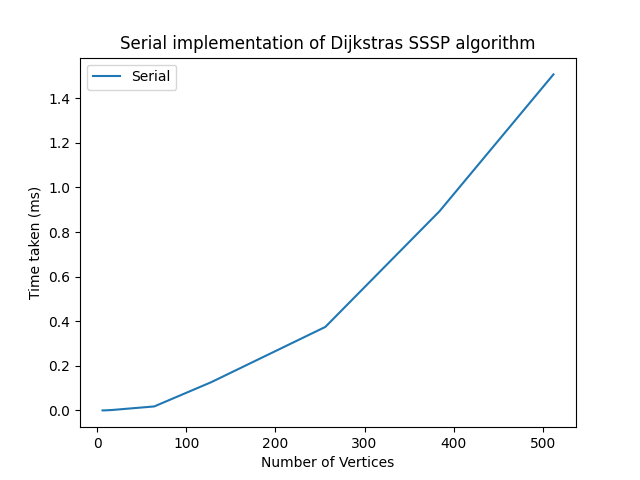
\includegraphics[width=0.6\linewidth]{serial_sssp.png}
		\caption{Serial SSSP algorithm average times}
		\label{fig:fig_serial_sssp}
	\end{figure}
	
	\subsection{OpenMP Parallel Implementation:}
	Next I implented the SSSP algorithm within OpenMP's interface. The approach I used is based off Dijkstra's SSSP iterative approach, while finding the minimum distance for each node gets assigned a thread to split the work done\cite{he2021parallelizing} given in Listing~\ref{listing:ls_sssp_omp}
	\begin{lstlisting}[caption={OpenMP Parallel algorithm for computing SSSP\cite{he2021parallelizing}}, label={listing:ls_sssp_omp}]
		int* dijkstra(int **graph, int src){
			int* dist = (int*)malloc(V * sizeof(int));
			dist[src] = 0; // Distance of source vertex from itself is always 0
			int i, md, mv;
			int my_first; // The first vertex that stores in one thread locally. 
			int my_id; // ID for threads
			int my_last; //The last vertex that stores in one thread locally. 
			int my_md; // local minimum distance
			int my_mv; // local minimum vertex
			int my_step; /* local vertex that is at the minimum distance from the source */
			int nth; /* number of threads */
			bool sptSet[V]; // sptSet[i] will be true if vertex i has been visited
			
			// Initialize all distances as INFINITE and stpSet[] as false
			for (i = 0; i < V; i++)
				dist[i] = INT_MAX, sptSet[i] = false;
			
			/* OpenMP parallelization starts here */
			#pragma omp parallel private ( my_first, my_id, my_last, my_md, my_mv, my_step )\
			shared ( src, md, dist, mv, nth, graph )
			{
				my_id = omp_get_thread_num ( );
				nth = omp_get_num_threads ( );
				my_first = (my_id * V) / nth;
				my_last = ((my_id + 1) * V) / nth - 1;
				for (my_step = 0; my_step < V-1; my_step++) {
					#pragma omp single
					{
						md = INT_MAX;
						mv = -1;
					}
					int k;
					my_md = INT_MAX;
					my_mv = -1;
					
					/* Each thread finds the minimum distance unconnected vertex inner of the graph */
					for (k = my_first; k <= my_last; k++) {
						if (!sptSet[k] && dist[k] <= my_md) {
							my_md = dist[k];
							my_mv = k;
						}
					}
					
					/* 'critical' specifies that code is only be executed on 
					* one thread at a time, because we need to determine the 
					* minimum of all the my_md here. */
					#pragma omp critical
					{
						if (my_md < md) {
							md = my_md;
							mv = my_mv;
						}
					}
					
					/* 'barrier' identifies a synchronization point at which threads in a 
					* parallel region will wait until all other threads in this section reach 
					* the same point. So that md and mv have the correct value. */
					#pragma omp barrier
					
					#pragma omp single
					{
						/* It means we find the vertex and set its status to true. */
						if (mv != - 1){
							sptSet[mv] = true;
						}
					}
					
					# pragma omp barrier
					
					if ( mv != -1 ){
						int j;
						for (j = my_first; j <= my_last; j++) {
							if (!sptSet[j] && graph[mv][j] && dist[mv] != INT_MAX
							&& dist[mv] + graph[mv][j] < dist[j])
							dist[j] = dist[mv] + graph[mv][j];
						}
					}
					#pragma omp barrier
				}
			}
			return dist;
		}
	\end{lstlisting}
	
	\newpage
	The algorithm works as follows:
	\begin{itemize}
		\item Initialize all variables
		\item Start omp parallel
		\item Private variables: $my\textunderscore first, my\textunderscore id, my\textunderscore last, my\textunderscore md, my\textunderscore mv, my\textunderscore step$
		\item Shared variables: $src, md, dist, mv, nth, graph$
		\item Set: $my\textunderscore id$ to current thread ID; $nth$ to total thread count; $my\textunderscore first$ to $(my\textunderscore id * V) / nth$; and $my\textunderscore last$ to $((my\textunderscore id + 1) * V) / nth - 1$;
		\item Begin a for loop (from $0$ to $V-1$)
		\item Begin an omp single contruct, set $md$ to an arbitrarily large number and $mv$ to non-existent $(-1)$
		\item Now set $my\textunderscore md$ and $my\textunderscore mv$ in the same way
		\item Begin a for loop from $my\textunderscore first$ to (and including) $my\textunderscore last$ 
		\item Inside the for loop, check 2 things: if node has been visited and if distance of node ($dist[k]$) is less than local minimum distance ($my\textunderscore md$)
		\item If true: set $my\textunderscore md = dist[k]$ and $my\textunderscore mv = k$
		\item Begin an omp critical construct, inside check if $my\textunderscore md < md$. If true: $md = my\textunderscore md$ and $mv = my\textunderscore mv$
		\item Initiate omp barrier
		\item Begin an omp single contruct, if $mv$ is not $-1$ then set node $mv$ to visited
		\item Initiate another omp barrier
		\item Check if $mv$ is not $-1$ then begin a for loop from $my\textunderscore first$ to (and including) $my\textunderscore last$ 
		\item Inisde the loop check 3 things: node$[j]$ not visited; cost at $[mv][j]$ and dist$[mv]$ are not the default large number we set; finally if dist$[mv]$ + cost at $[mv][j]$ are less than dist$[j]$
		\item If all conditions are met, set dist$[j]$ = dist$[mv]$ + cost at $[mv][j]$
		\item After the for loop initiate omp barrier
		\item Return the distance array
	\end{itemize}
	
	I experimented with different number of threads running and noticed any number of threads less than 6 produce similar results. While anything over 6 starts to slow down the algorithm rather than speed it up. From this conclusion I chose thread counts of $2,3,4$ to compare, given in Figure~\ref{fig:fig_sssp_omp}
	\begin{figure}[!htb]
		\centering
		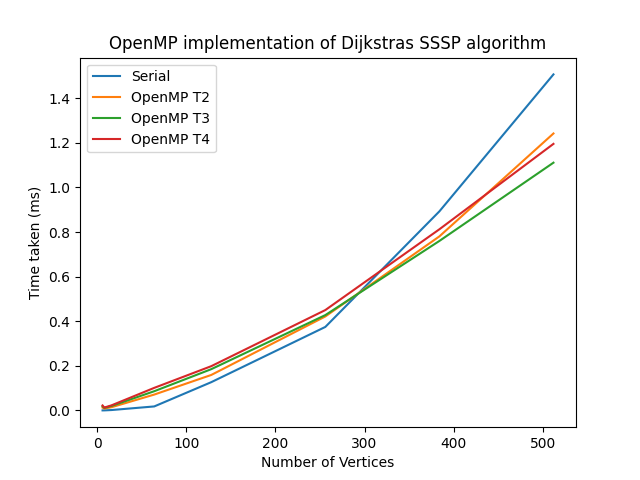
\includegraphics[width=0.6\linewidth]{sssp_omp.png}
		\caption{OpenMP Parallel SSSP algorithm average times for different thread counts}
		\label{fig:fig_sssp_omp}
	\end{figure}

	All 3 parallel implementations deviate very slightly from eachother. In parallel speedup is only noticed at around 250 vertices and higher, otherwise serial performs better. With 3 threads running there is a slightly better speedup at higher vertex counts.
	
	\subsection{MPI Parallel Implementation:}
	Next I implented the SSSP algorithm within MPI's interface. The approach I used is based off Dijkstra's SSSP iterative approach, while finding the minimum distance for each node gets assigned a thread to split the work done\cite{he2021parallelizing} given in Listing~\ref{listing:ls_sssp_mpi}
	\begin{lstlisting}[caption={MPI Parallel algorithm for computing SSSP\cite{he2021parallelizing}}, label={listing:ls_sssp_mpi}]
		void SingleSource(int source, int *wgt, int *lengths, MPI_Comm comm) {
			int i, j;
			int nlocal; /* The number of vertices stored locally */
			int *marker; /* Used to mark the vertices belonging to Vo */
			int firstvtx; /* The index of the first local vertex */
			int lastvtx; /* The index of the last local vertex */
			int u, udist;
			int lminpair[2], gminpair[2];
			int npes, myrank;
			
			MPI_Comm_size(comm, &npes);
			MPI_Comm_rank(comm, &myrank);
			
			nlocal = V / npes;
			firstvtx = myrank*nlocal;
			lastvtx = firstvtx + nlocal - 1;
			
			/* Set the initial distances from source to all the other vertices */
			for (j = 0; j<nlocal; j++) {
				lengths[j] = wgt[source*nlocal + j];
			}
			/* This array is used to indicate if the shortest part to a vertex has been found or not. */
			/* if marker [v] is one, then the shortest path to v has been found, otherwise it has not. */
			marker = (int *)malloc(nlocal*sizeof(int));
			for (j = 0; j<nlocal; j++) {
				marker[j] = 1;
			}
			
			/* The process that stores the source vertex, mark as seen */
			if (source >= firstvtx && source <= lastvtx) {
				marker[source - firstvtx] = 0;
			}
			
			/* The main loop of Dijkstra's algorithm */
			for (i = 1; i<V; i++) {
				/* Step 1: Find local vertex with smallest distance from source */
				lminpair[0] = INT_MAX; /* set it to an arbitrarily large number */
				lminpair[1] = -1;
				for (j = 0; j<nlocal; j++) {
					if (marker[j] && lengths[j] < lminpair[0]) {
						lminpair[0] = lengths[j];
						lminpair[1] = firstvtx + j;
					}
				}
				
				/* Step 2: Compute the global minimum vertex, insert it into Vc */
				MPI_Allreduce(lminpair, gminpair, 1, MPI_2INT, MPI_MINLOC, comm);
				udist = gminpair[0];
				u = gminpair[1];
				/* The process that stores the minimum vertex, mark as seen */
				if (u == lminpair[1]) {
					marker[u - firstvtx] = 0;
				}
				
				/* Step 3: Update the distances given that u got inserted */
				for (j = 0; j<nlocal; j++) {
					if (marker[j] && ((udist + wgt[u*nlocal + j]) < lengths[j])
					&& wgt[u*nlocal + j] != INT_MAX && udist != INT_MAX) {
						lengths[j] = udist + wgt[u*nlocal + j];
					}
				}
			}
			if (myrank == 0) free(marker);
		}
	
		int main(int argc, char *argv[]) {
			int npes, myrank, nlocal;
			int i, j, k;
			int *localWeight; /*local weight array*/
			int *localDistance; /*local distance vector*/
			
			MPI_Init(&argc, &argv);
			MPI_Comm_size(MPI_COMM_WORLD, &npes);
			MPI_Comm_rank(MPI_COMM_WORLD, &myrank);
			
			nlocal = V/npes; /* number of elements per thread. */
			
			int graph[V*V];
			int sendbuf[V*V]; /*local weight to distribute*/
			int dist = (int*)malloc(V * sizeof(int)); /*distance vector*/
			
			localWeight = (int *)malloc(nlocal*V*sizeof(int));
			localDistance = (int *)malloc(nlocal*sizeof(int));
			
			/*prepare send data */
			for(k=0; k<npes; ++k) {
				for(i=0; i<V;++i) {
					for(j=0; j<nlocal;++j) {
						sendbuf[k*V*nlocal+i*nlocal+j]=graph[i][k*nlocal+j];
					}
				}
			}
		
			/*distribute data*/
			MPI_Scatter(sendbuf, nlocal*V, MPI_INT, localWeight, nlocal*V, MPI_INT,
			0, MPI_COMM_WORLD); 
			
			/*Implement the single source dijkstra's algorithm*/
			SingleSource(0, localWeight, localDistance, MPI_COMM_WORLD);
			
			/*collect local distance vector at the source process*/
			MPI_Gather(localDistance, nlocal, MPI_INT, dist, nlocal, MPI_INT, 
			0, MPI_COMM_WORLD);
			
			MPI_Finalize();
		}
	\end{lstlisting}
	
	\newpage
	The algorithm works as follows:
	\begin{itemize}
		\item Initialize all global variables
		\item Start MPI
		\item Get comm rank and size
		\item Set number of local vertices to total vertices ($V$) / comm size ($npes$)
		\item Initialize more variables
		\item Prepare to send localized data
		\item Distribute data with MPI call Scatter\cite{MPIScatter}
		\item Implement Dijkstra's SSSP algorithm in parallel
		\begin{itemize}
			\item Initialize all local variables
			\item Get comm rank and size
			\item Set number of local vertices to total vertices ($V$) / comm size ($npes$)
			\item Set starting vertex and ending vertex for current process
			\item Get initial distances from source to all other vertices
			\item Initialize a marker array
			\item Mark the source as seen
			\item Find local minimum distances per process
			\item Find global minimum distance and insert it into $V_c$
			\item MPI call to Allreduce\cite{MPIAllreduce}
			\item Mark the vertex with the minimum distance as seen
			\item Update all distances from local to global
			\item Free marker array from memory
		\end{itemize}
		\item Collect distance data with MPI call Gather\cite{MPIGather}
		\item End MPI
	\end{itemize}
	
	I experimented with different number of threads running and noticed number of threads less than 6 produce desired speedup. While anything over 6 starts to slow down the algorithm rather than speed it up. From this conclusion I chose thread counts of $2,3,6$ to compare, given in Figure~\ref{fig:fig_sssp_mpi}
	\begin{figure}[!htb]
		\centering
		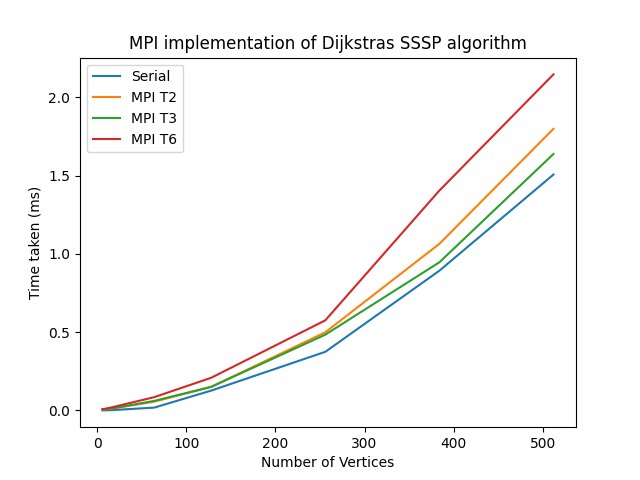
\includegraphics[width=0.6\linewidth]{sssp_mpi.png}
		\caption{MPI Parallel SSSP algorithm average times for different thread counts}
		\label{fig:fig_sssp_mpi}
	\end{figure}
	
	All 3 parallel implementations perform quite similarly. With noticeable trends, in 6 threads, speedup is only achieved at 250 vertices and higher, while 2 and 3 threads achieve speedup much earlier. With 3 threads running there is consistently more speedup at all vertex counts.
	
	\newpage
	\subsection{Validation:}
	Comparing output with serial counterpart, through running $run.sh$ given in Figure~\ref{fig:fig_sssp_validation}
	\begin{figure}[!htb]
		\centering
		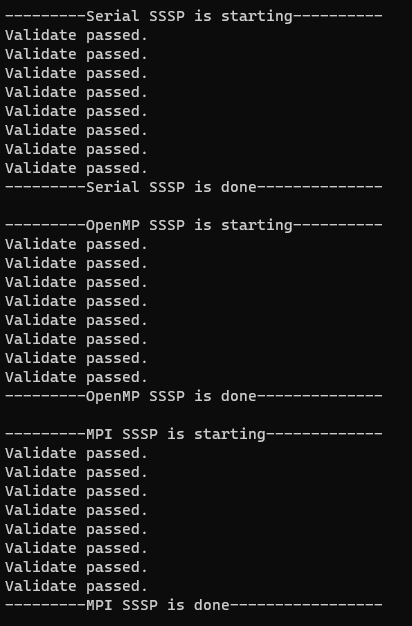
\includegraphics[height=0.5\linewidth]{sssp_validation.png}
		\caption{Validation of SSSP operations}
		\label{fig:fig_sssp_validation}
	\end{figure}

	\subsection{Conclusions:}
	After comparing the results from serial, optimal OpenMP (with 3 threads) and optimal MPI (with 3 threads), I can make the conclusion that speedup at small vertex counts is negligible. While around the 250 vertex count mark, both OpenMP and MPI have significant speedup from serial, with MPI speedup being consistently better than OpenMP.
	Comparisons given in Figure~\ref{fig:fig_sssp_comparison}
	\begin{figure}[!htb]
		\centering
		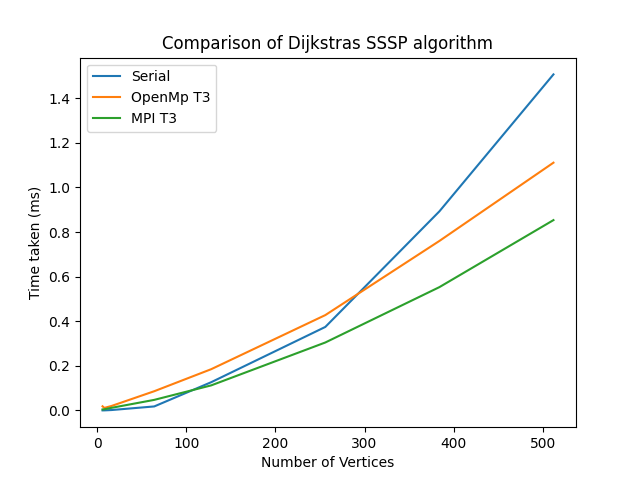
\includegraphics[width=0.6\linewidth]{sssp_comparison.png}
		\caption{Comparison of all scan operations}
		\label{fig:fig_sssp_comparison}
	\end{figure}

	The speedup is given in Table~\ref{tab:example}.
	\begin{table}[!htb]
		\centering
		\caption{Table of speedup (in ms)}\label{tab:example}
		\begin{tabular}{l|cccccccc}
			\toprule
			No of vertices & 6 & 8 & 16 & 64 & 128 & 256& 384 & 512\\
			\midrule
			Serial &0.0002&0.0003&0.0018&0.0180&0.1268&0.3746&0.8928&1.5070\\
			Parallel &0.0046&0.0052&0.0117&0.0474&0.1125&0.3048&0.5530&0.8536\\
			Sppedup &0&0&0&0&1.13&1.23&1.62&1.77\\
			\bottomrule
		\end{tabular}
	\end{table} 
	
	\newpage
	\bibliography{main}
	
\end{document} 

